%
% File acl2014.tex
%
% Contact: koller@ling.uni-potsdam.de, yusuke@nii.ac.jp
%%
%% Based on the style files for ACL-2013, which were, in turn,
%% Based on the style files for ACL-2012, which were, in turn,
%% based on the style files for ACL-2011, which were, in turn, 
%% based on the style files for ACL-2010, which were, in turn, 
%% based on the style files for ACL-IJCNLP-2009, which were, in turn,
%% based on the style files for EACL-2009 and IJCNLP-2008...

%% Based on the style files for EACL 2006 by 
%%e.agirre@ehu.es or Sergi.Balari@uab.es
%% and that of ACL 08 by Joakim Nivre and Noah Smith

\documentclass[11pt]{article}
\usepackage{acl2014}
\usepackage{times}
\usepackage{url}
\usepackage{latexsym}


%%%%%% ADDED TO GET CORRECT PDF SIZE
\pdfpagewidth=\paperwidth
\pdfpageheight=\paperheight


%%%%%% EXTRA PACKAGES
\usepackage{graphicx}
\usepackage{listings}
\usepackage{tabularx}
\usepackage{ctable}
\usepackage{booktabs}


%\setlength\titlebox{5cm}

% You can expand the titlebox if you need extra space
% to show all the authors. Please do not make the titlebox
% smaller than 5cm (the original size); we will check this
% in the camera-ready version and ask you to change it back.


\title{\textit{lex4all}: A language-independent tool for building and evaluating pronunciation lexicons for small-vocabulary speech recognition}

%\author{Anjana Vakil \\
%  Affiliation / Address line 1 \\
%  Affiliation / Address line 2 \\
%  Affiliation / Address line 3 \\
%  {\tt email@domain} \\\And
%  Max Paulus \\
%  Affiliation / Address line 1 \\
%  Affiliation / Address line 2 \\
%  Affiliation / Address line 3 \\
%  {\tt email@domain} \\}

\date{}

\begin{document}
\maketitle

\begin{abstract}
This paper describes \textit{lex4all}, an open-source PC application for the generation and evaluation of pronunciation lexicons in any language. With just a few minutes of recorded audio and no expert knowledge of linguistics or speech technology, individuals or organizations seeking to create speech-driven applications in low-resource languages can use this tool to build pronunciation lexicons enabling small-vocabulary speech recognition in the target language using a high-quality commercial recognition engine designed for a high-resource source language (e.g. English). This is possible thanks to an existing algorithm for cross-language phoneme-mapping; we give an overview of this method and describe its implementation in \textit{lex4all}. Beyond the core functionality of building new lexicons, the tool also offers a built-in audio recorder that facilitates data collection, and an evaluation module that simplifies and expedites research on small-vocabulary speech recognition using cross-language mapping. 
%Finally, we report on an investigation into the impact of varying the high-resource source language used; our results seem to indicate that phonetic similarity between target and source language does not significantly affect recognition accuracy, underscoring the system's language-independence.
\end{abstract}


%Demo submissions should also clearly indicate if any computer equipment is expected to be provided by the local organizer. If so, please specify desired hardware platform, hard disk and memory capacity, operating system and other software needed in order to run the demo. 
%
%Implementation of ACL multiple submission policy: Papers being submitted both to ACL and another conference or workshop must
%\begin{itemize}
%\item Note on the title page the other conference or workshop to which they are being submitted. (This includes submissions that are extensions of papers currently being submitted to a workshop.)
%\item State on the title page that if the paper is accepted for ACL, then the paper will be withdrawn from other conferences and workshops.
%\end{itemize}
%Papers that overlap other papers that have appeared at a conference with published proceedings must contain significant new results. Authors must include on the title page a list of any previous papers that the current paper overlaps or extends, and must identify the significant new results contained in the new submission. The program co-chairs have the final decision about what constitutes significant new results.

\section{Introduction\footnote{Parts of this paper (Sections \ref{sec:intro} and \ref{sec:background}) overlap with a paper submitted to the 4th Workshop on Spoken Language Technologies for Under-resourced languages (SLTU '14, \url{http://www.mica.edu.vn/sltu2014}). That paper, which is currently under review, concerns related research not reported here, and makes no mention of the lex4all application.}}
\label{sec:intro}

In recent years it has been demonstrated that speech recognition interfaces can be extremely beneficial for applications in the developing world, particularly in communities where literacy rates are low or where PCs and internet connections are not always available \cite{case4st4d,bali13,Sherwani09}. 
Typically, the languages spoken in such communities are under-resourced, such that the large audio corpora typically needed to train or adapt recognition engines are unavailable.
%, and collecting such vast amounts of data is generally infeasible for individuals or small organizations interested in developing speech-driven applications for their communities. 
However, in the absence of a recognition engine trained for the target low-resource language (LRL), an existing recognizer for a completely unrelated high-resource language (HRL), such as English, can be used to perform small-vocabulary recognition tasks in the LRL. 
%(By ``small-vocabulary tasks'' we mean those requiring discrimination between a few dozen terms.) 
%of the type required in grammar-controlled applications (e.g. for accessing information or conducting basic transactions), which may require the system to distinguish a few dozen terms in the URL. 
All that is needed is a pronunciation lexicon mapping each term in the target vocabulary to one or more sequences of phonemes in the HRL, i.e. phonemes which the recognizer can model. 

This is the motivation behind \textit{lex4all}, an open-source desktop application for Windows that allows users to automatically create a mapped pronunciation lexicon for words in any language, using a small number of audio recordings and a pre-existing recognition engine in a HRL such as English. The resulting lexicon can then be used with the HRL recognizer to add small-vocabulary speech recognition functionality to applications in the LRL, without the need for the large amounts of data and expertise in speech technologies required to train a new recognizer. This paper describes the \textit{lex4all} application and its utility as a tool for rapid, simple creation and evaluation of mapped pronunciation lexicons for small-vocabulary speech recognition in any language.

\section{Background and related work}
\label{sec:background}
Many commercial speech recognition systems offer high-level Application Programming Interfaces (APIs) that make adding voice recognition capabilities to an application as simple as specifying (in text) the words/phrases that should be recognized; this requires very little general technical expertise, and virtually no knowledge of the inner workings of the recognition engine. If the target language is supported by the system -- the Microsoft Speech Platform, for example, currently supports recognition and synthesis for 26 languages/dialects \cite{mspsdk} -- this makes it very easy for small-scale software developers (i.e. individuals or small organizations without much funding) to create new speech-driven applications. 

While many such individuals or organizations in the developing world may be interested in using such platforms to create speech-driven applications for use in their communities, the low-resource languages typically spoken in these areas are obviously not supported by such commercial systems. 
And though many effective techniques for training or adapting recognizers for new languages exist (see e.g. the CMUSphinx toolkit\footnote{\url{http://www.cmusphinx.org}} or the Rapid Language Adaptation Toolkit\footnote{\url{http://i19pc5.ira.uka.de/rlat-dev}}), these typically require hours of training audio to produce effective models, and even the highest-level tools for building new models still require a nontrivial amount of expertise with speech technologies; such data and expertise may not be available to the small-scale developers in question.

However, many useful development-oriented applications (e.g. for accessing information or conducting basic transactions) require only small-vocabulary recognition tasks, by which we mean those requiring discrimination between a few dozen terms.
For such tasks, an unmodified HRL recognizer can be used as-is to perform recognition of the LRL terms; as Figure~\ref{fig:background} illustrates, we simply need an application-specific grammar describing the allowable combinations and sequences of words/phrases to be recognized, and a pronunciation lexicon which maps each of the target words/phrases to a sequence of phonemes in the source language for which the recognizer has been trained (see Listing~\ref{lst:lexicon} for an example). 

\begin{figure}[tb]
\begin{center}
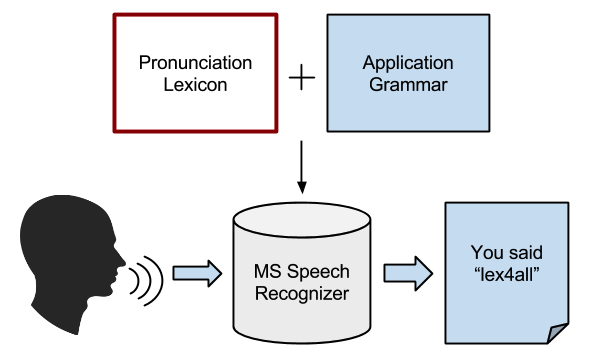
\includegraphics[width=\columnwidth]{../img/background-diagram-cropped.png}
\caption{Given a pronunciation lexicon and application-specific grammar, an existing recognizer for a HRL can be used to recognize speech in a LRL.\label{fig:background}}
\end{center}
\end{figure}

%Listing~\ref{lst:lexicon} shows a sample lexicon XML file conforming to the Pronunciation Lexicon Specification \cite{pls}. A lexicon is composed of one \texttt{lexeme} element for each term-sound pairing. In a lexicon intended for speech recognition, each \texttt{lexeme} consists of one \texttt{grapheme} element, representing the term's orthographic form, and one or more \texttt{phoneme} elements, each containing a sequence of phonemes that constitutes an acceptable pronunciation of the term. 

\lstset{
	%language=xml,
	basicstyle={\footnotesize\ttfamily},
	%frame=tb,
	numbers=none,
	linewidth=\columnwidth,
	breaklines=true,
	captionpos=b,
	}
\begin{figure}
\begin{lstlisting}[caption=\texttt{lexicon.pls}: A sample lexicon mapping Yoruba words to American English pronunciations.]
<?xml version="1.0" encoding="utf-8" standalone="no"?>
	  
<lexicon version="1.0" xmlns="http://www.w3.org/2005/01/pronunciation-lexicon" xml:lang="en-US" alphabet="x-microsoft-ups">
		 
  <lexeme>
    <grapheme>mefa</grapheme>
    <phoneme>M EH F AX</phoneme>
  </lexeme>
  
  <lexeme>
    <grapheme>beeni</grapheme>
    <phoneme>B E NG I</phoneme>
  </lexeme>
  
</lexicon>
\end{lstlisting}
\label{lst:lexicon}
\end{figure}

This is the thinking behind Speech-based Automated Learning of Accent and Articulation Mapping, or ``Salaam'' \cite{Sherwani09,Qiao10,Chan12}. This method of cross-language phoneme-mapping enables the automatic discovery of source-language pronunciation sequences for words or phrases in the (unrelated) target language, and thus constitutes the foundation on which the lex4all tool is built.

The basic idea of phoneme-mapping is to discover the best pronunciation sequence for a given word in the target language by using the source language recognizer to perform phone decoding on one or more audio samples of the target word. However, the APIs for commercial recognizers such as Microsoft's are designed for word-decoding, and do not usually enable the use of the phone-decoding mode. The insight of the Salaam approach is to use a specially designed grammar to mimic this phone decoding \cite[\S3.2]{Chan12}. 
Specifically, Qiao et al. \cite[§4.1]{Qiao10} create a recognition grammar representing a phoneme ``super-wildcard'' that guides pronunciation discovery. 
This grammar allows the recognizer to treat an audio sample of the target word as a ``phrase'' made up of 0-10 ``words'',
where each ``word'' can be matched to any possible sequence of 1, 2, or 3 source language phonemes \cite[§4.1]{Qiao10}. 

Given this super-wildcard grammar and one or more audio recordings of the target word, Qiao et al. \cite[§4.1]{Qiao10} use an iterative training algorithm to discover the best pronunciation(s) for that word, one phoneme at a time. 
In the first pass, the recognizer finds the best match(es) for the first phoneme, then for the first two phonemes in the second pass, and so on until a stopping criterion is met, e.g. the recognition confidence score assigned to the resulting ``phrase'' stops improving \cite[p.~4]{Qiao10}.

Compared to expert-crafted pronunciations, using pronunciations generated automatically by this algorithm improves recognition accuracy substantially \cite[§5.2]{Qiao10}. By training on samples from two speakers instead of one, and by using a pronunciation lexicon containing multiple pronunciations for each word (i.e. the $n$-best results of the training algorithm instead of the single best result), Qiao et al. are able to further improve accuracy. Chan and Rosenfeld \cite{Chan12} achieve still higher accuracy by applying an iterative discriminative training algorithm, identifying and removing pronunciations that cause confusion between word types.

In sum, the Salaam method is fully automatic, requiring expertise neither in speech technology (to modify acoustic models) nor in linguistics (to manually generate seed pronunciations), and for each new target language it requires only a few minutes' worth of training data from one or more speakers, an amount that can be collected in a short time with little effort or expense. At the same time, it enables the construction of pronunciation lexicons that can help bring speech recognition applications to LRLs. This has been demonstrated in at least two developing-world projects that have successfully used the Salaam method to add voice interfaces to real applications: an Urdu telephone-based health information system in Pakistan \cite{Sherwani09}, and a text-free Hindi smartphone application to deliver agricultural information to farmers in rural India \cite{bali13}.


Given the established success of the Salaam method for pronunciation discovery, our contribution is to build an easy-to-use graphical application around these algorithms, so that non-expert users can quickly and easily create the pronunciation lexicons necessary for developing speech interfaces in LRLs using existing HRL recognizers. In the following sections, we describe the lex4all application and the modified implementation of the Salaam method which is at its core.


\section{System overview}
\label{sec:overview}

\begin{figure}[t]
\begin{center}
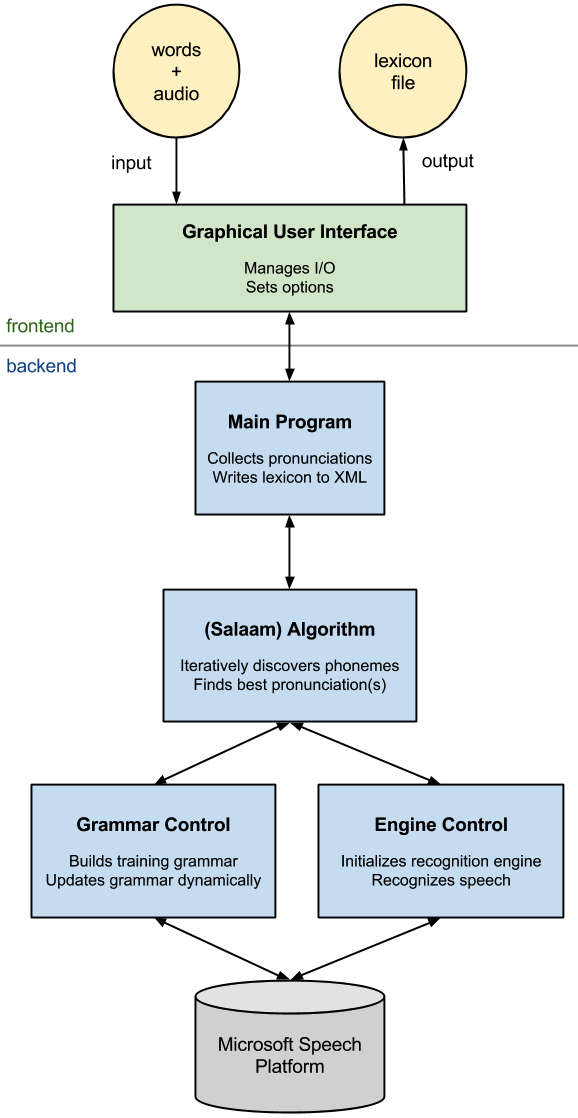
\includegraphics[width=\columnwidth]{../img/SystemOverview.png}
\caption{Overview of the core components of the lex4all lexicon-building system.\label{fig:system}}
\end{center}
\end{figure}

(TODO: CHANGE THIS TEXT)
A simple user interface allows the user to easily specify one written form (text string) and and one or more audio samples (.wav files) for each word in the target vocabulary, and to set other options (e.g. number of pronunciations per word, name/save location of lexicon file, etc.). The audio is then passed to a speech recognition engine for a HRL (English). An automatic pronunciation generation algorithm (the Salaam method) finds the best pronunciation(s) for each word in the LRL vocabulary. The program outputs a pronunciation lexicon (.pls XML file). This lexicon file follows the standard pronunciation lexicon format \cite{pls}, so it can be directly included in a speech recognition application, e.g. one built using the Microsoft Speech Platform API.



\section{User interface}
\label{sec:frontend}
Easy for non-experts (include informative screenshot)

Audio input: use existing or new

\subsection{Audio recording}
\label{sec:recording}

Things to mention (Max, please add to this):
\begin{itemize}
\item{NAudio}
\end{itemize}



\section{Pronunciation mapping}
\label{sec:backend}

\subsection{Implementation of the Salaam method}
\label{sec:implementation}
\cite{Qiao10}

\subsection{Running time}
\label{sec:runningtime}

Text goes here

\begin{table*}[tb]
\begin{center}

\begin{tabular}{lrccrr}
%{
%\toprule
 &  & \multicolumn{2}{c}{Mean Accuracy (\%)} & Difference & $p$-value \\
\cmidrule(rl){3-4}
& & Old wildcard & New wildcard & &  \\
\midrule
\addlinespace
Same-speaker & Female (avg.) & 72.8 & \textbf{73.6} &+0.8 & 0.75 \\
(leave-one-out)		& Male (avg.) & \textbf{90.4} & \textbf{90.4} & 0.0 & 1.00 \\
			& Overall average & 81.6 & \textbf{82} &  +0.4 & 0.81 \\
\addlinespace
\addlinespace

%\midrule
\addlinespace
Cross-speaker	&Male $\rightarrow$ Female & \textbf{70.4} & 66.4 & -4.0 & \\
(train $\rightarrow$ test)		& Female $\rightarrow$ male & 76.8 & \textbf{77.6}& +0.8	&  \\
			&Average & \textbf{73.6} & 72 	&-1.6	& 0.63 \\
\addlinespace
%\addlinespace
\midrule
%}
\end{tabular}
\end{center}
\caption{Word recognition accuracy using American English recognizer on Yoruba audio (25~words, 2~speakers, 5~samples per word per speaker), with results of paired two-tailed $t$-test for significance.\label{tab:accuracy}}
\end{table*}



\subsection{Discriminative training}
\label{sec:discrimtrain}
\cite{Chan12}


\section{Evaluation module for research}
\label{sec:evaluation}

\section{Conclusion and future work}
\label{sec:future}




%\section*{Acknowledgments}
%
%The acknowledgments should go immediately before the references.  Do
%not number the acknowledgments section. Do not include this section
%when submitting your paper for review.

% include your own bib file like this:
%\bibliographystyle{acl}
%\bibliography{acl2014}
\bibliographystyle{acl}
\bibliography{lex4all.bib}


\end{document}
